\documentclass{standalone}
\usepackage[utf8]{inputenc}
\usepackage{pgfplots}
\DeclareUnicodeCharacter{2212}{−}
\usepgfplotslibrary{groupplots,dateplot}
\usetikzlibrary{patterns,shapes.arrows}
\pgfplotsset{compat=newest}
\begin{document}
% This file was created with tikzplotlib v0.10.1.
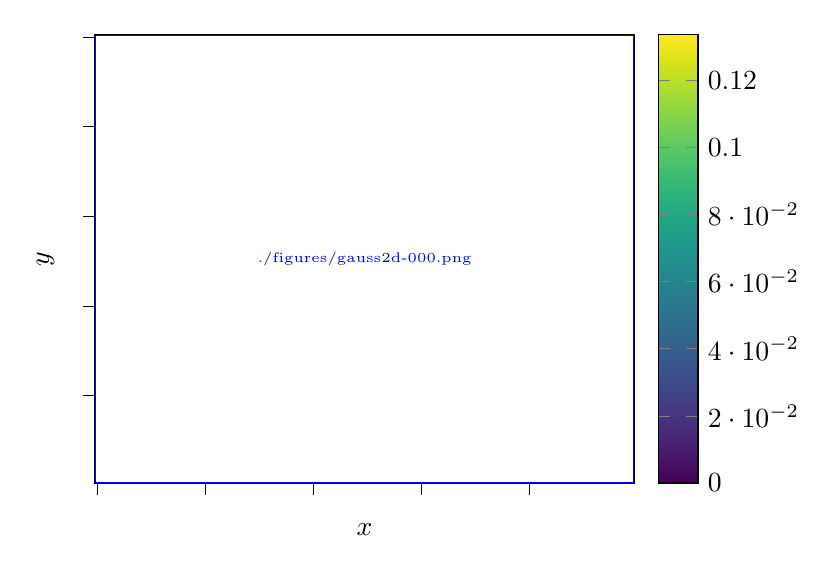
\begin{tikzpicture}

\definecolor{darkgray176}{RGB}{176,176,176}

\begin{axis}[
colorbar,
colorbar style={ylabel={}},
colormap/viridis,
point meta max=0.133614519080726,
point meta min=1.50608999074453e-08,
tick align=outside,
tick pos=left,
x grid style={darkgray176},
xmin=-0.5, xmax=99.5,
xtick style={color=black},
y dir=reverse,
y grid style={darkgray176},
ymin=-0.5, ymax=99.5,
ytick style={color=black},
xlabel={$x$},
ylabel={$y$},
xticklabels={,,},
yticklabels={,,}
]
\addplot graphics [includegraphics cmd=\pgfimage,xmin=-0.5, xmax=99.5, ymin=99.5, ymax=-0.5] {./figures/gauss2d-000.png};
\end{axis}

\end{tikzpicture}

\end{document}